% 08-architecture-et-exercices.tex — Réalisation 2/4 : architecture du site et
% exercices, avec l'exemple détaillé du looping avec wagon (≈ 8 pages).

\chapter{Architecture du site et exercices}
\label{chap:architecture}

\section{Organisation du code}

\begin{arediger}{1,5 page}
Un dossier par thème, un sous-dossier par exercice contenant exactement
\fichier{index.html}, \fichier{calcul.js} (physique pure, testable sous Node),
\fichier{main.js} (affichage et interactions) et éventuellement
\fichier{game.js}. Code visuel partagé (\fichier{canvas\_draw.js},
\fichier{graph\_plot.js}) mais jamais la physique. Scripts classiques exposant
un seul objet global, condition pour fonctionner en \fichier{file://}.
Schéma TikZ des dépendances entre fichiers.
\end{arediger}

\section{Gabarit commun d'une page}

\begin{arediger}{1,5 page}
Scène (canevas redessiné à chaque image), panneau de transport (lecture,
pause, vitesse \(\times 0{,}5\) à \(\times 4\), curseur temporel), paramètres
(curseur + champ numérique), formules, graphes. Bilingue FR/EN. Présenter
brièvement les exercices existants (tir parabolique, pendule, MCU, looping).
\end{arediger}

\section{Exemple détaillé : le looping avec wagon}
\label{sec:exercice-wagon}

La dernière version du looping a été conçue pour tenir sur un seul écran
(figure~\ref{fig:wagon-ecran}). Le rail est entièrement proportionnel au rayon
\(R\) du looping : rampe à \ang{60} partant de \(3R\), raccord circulaire de rayon
\(R\), piste de longueur \(R\), cercle de rayon \(R\). La vue est donc un cadre
fixe exprimé en unités de \(R\) : changer \(R\) ne change que l'échelle de la
grille, l'image ne bouge jamais et l'étudiant ne peut ni zoomer ni se déplacer.
Cette propriété permet de placer dans l'espace libre du canevas le diagramme des
forces, les barres d'énergie \(E_c\), \(E_p\), \(E_m\) et un état en direct
(position sur le rail, \(v\), \(N\), facteur de charge \(n\), verdict).

\begin{figure}[ht]
  \centering
  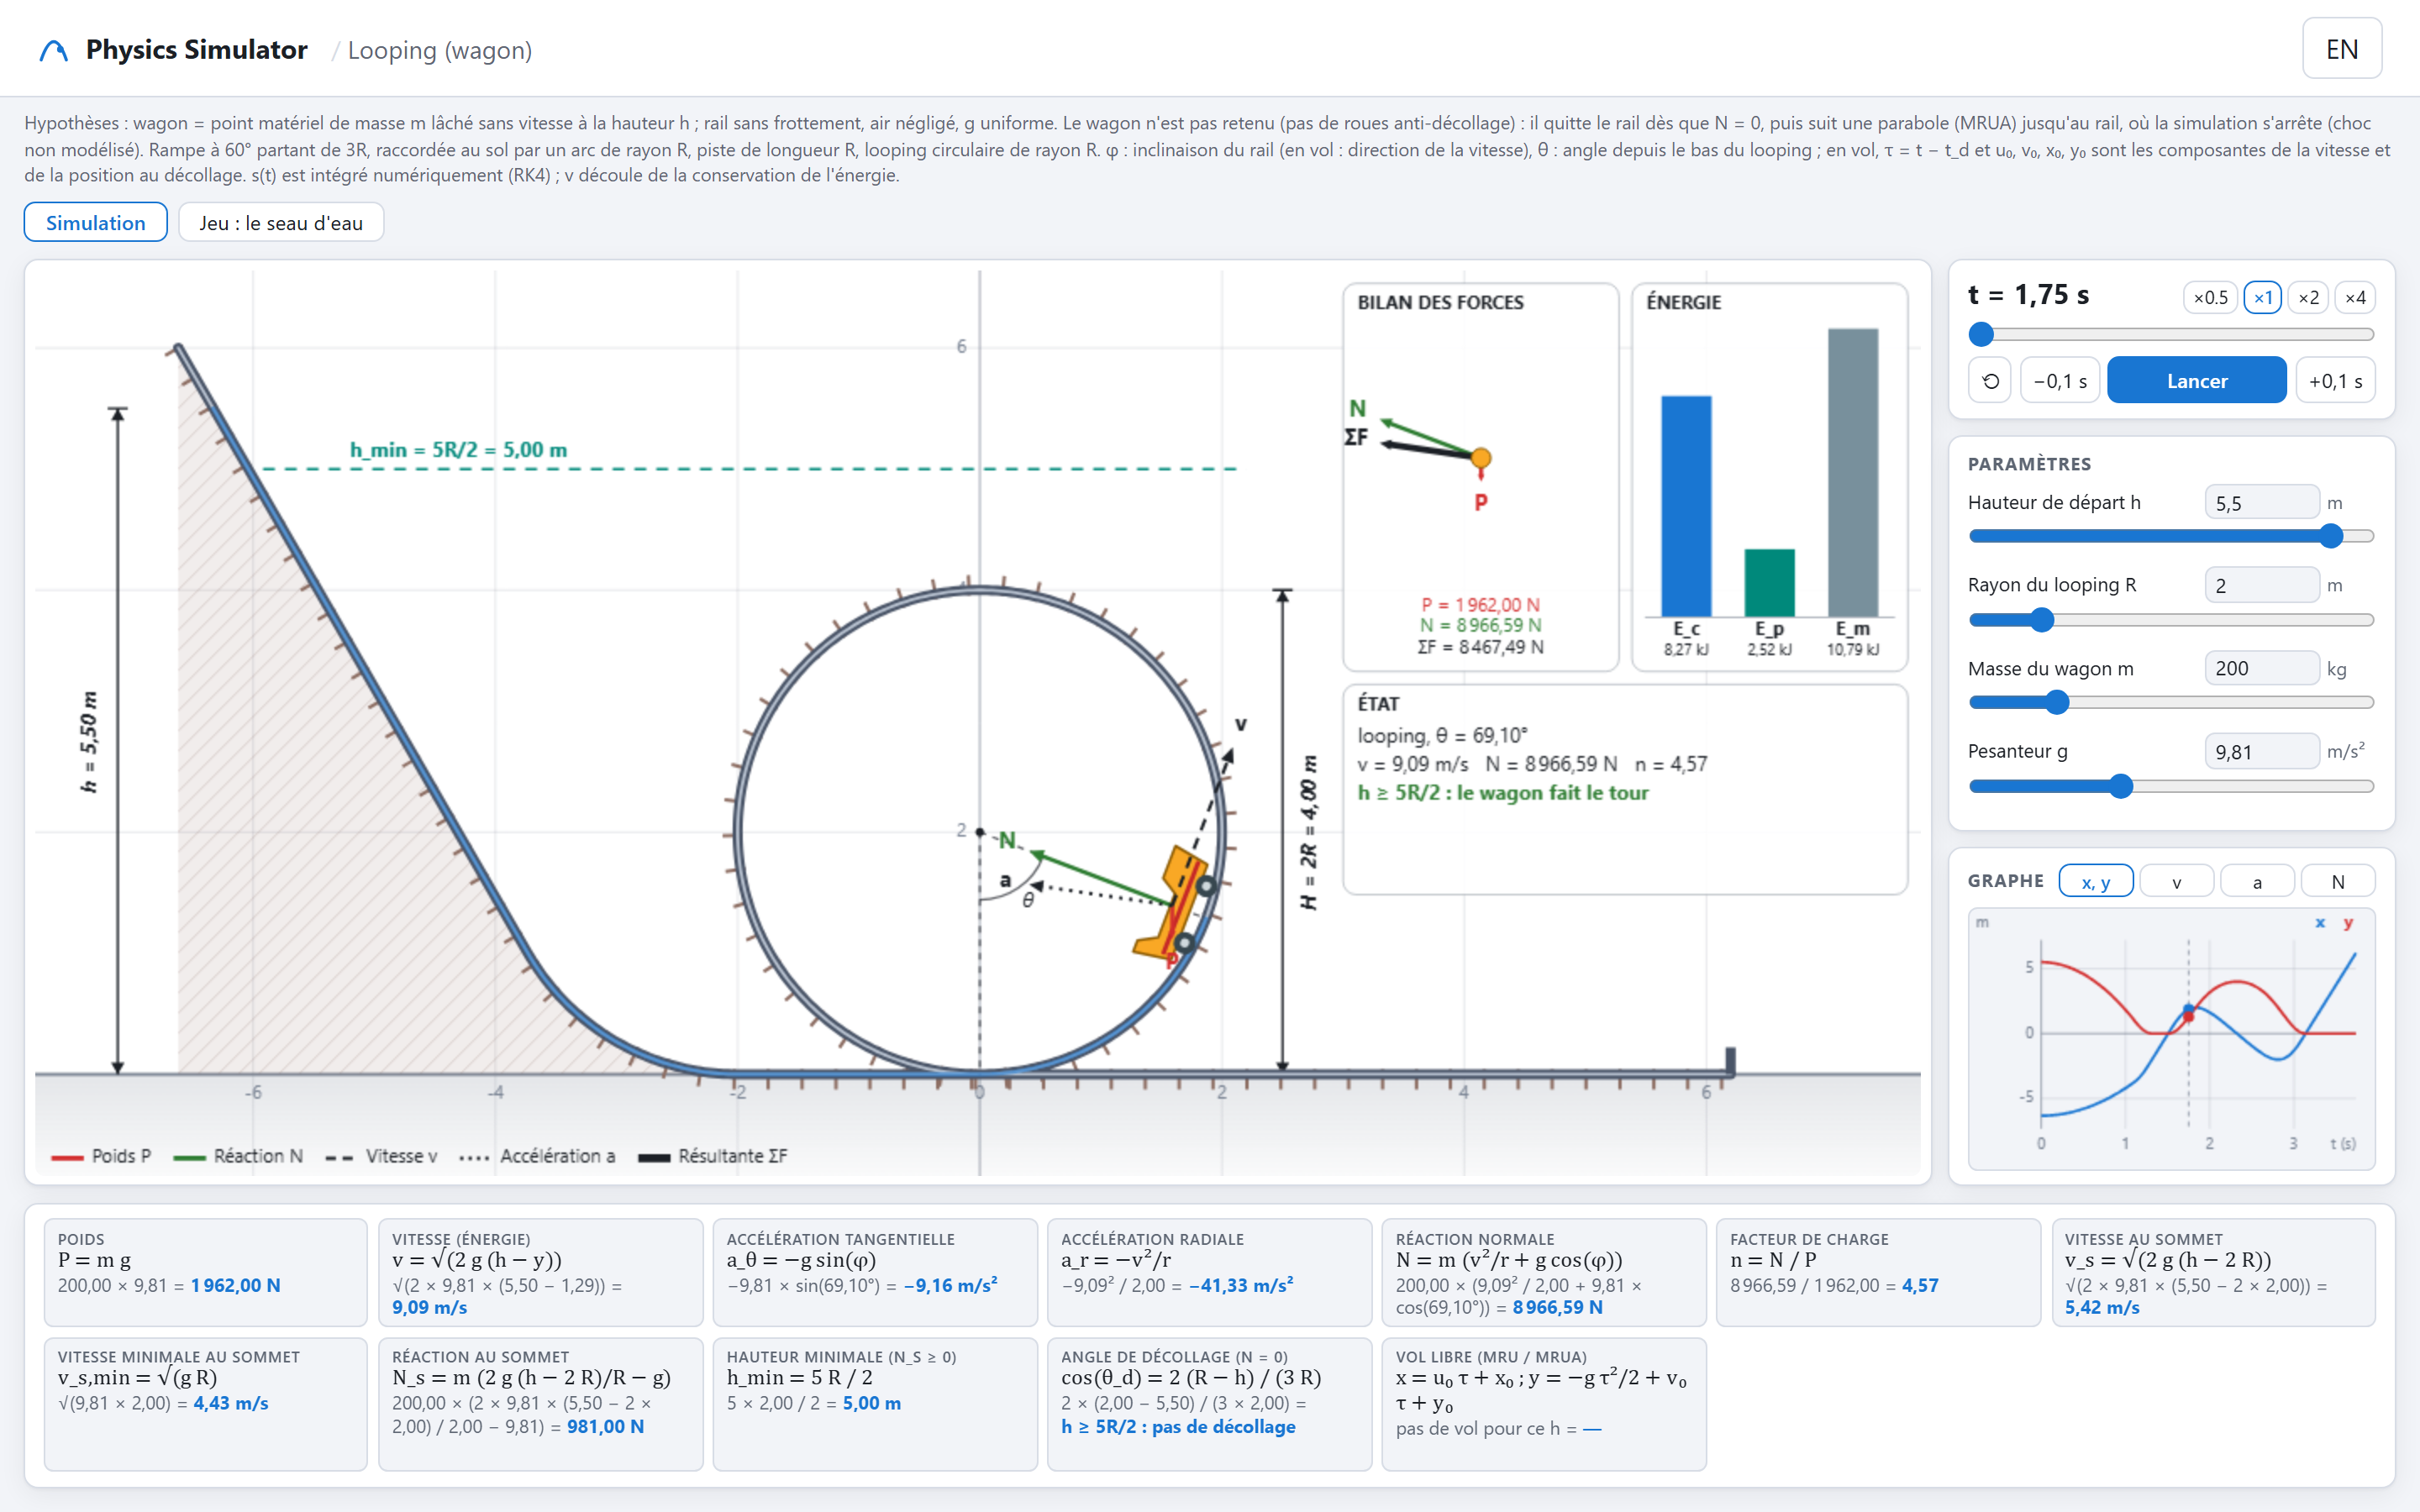
\includegraphics[width=\linewidth]{figures/captures/looping-ecran-complet.png}
  \caption{Exercice du looping avec wagon sur un écran de \(1440 \times 900\)
    pixels : scène avec vecteurs \(P\), \(N\), \(v\), \(a\), diagramme des forces,
    énergies et état dans l'espace libre du canevas ; transport, paramètres et
    graphe à droite ; douze formules substituées en bas.}
  \label{fig:wagon-ecran}
\end{figure}

\begin{arediger}{3 pages}
Rédiger : (1) le modèle (point matériel, rail sans frottement, wagon non
retenu) et les équations affichées : \(v = \sqrt{2 g (h - y)}\),
\(a_\theta = -g \sin(\varphi)\), \(a_r = -v^2/r\),
\(N = m (v^2/r + g \cos(\varphi))\), \(n = N/P\),
\(v_s = \sqrt{2 g (h - 2R)} \geq \sqrt{g R}\), \(h_{\min} = 5R/2\),
\(\cos(\theta_d) = 2 (R - h)/(3 R)\), vol libre en MRU/MRUA ; (2) les trois
régimes (le wagon fait le tour, décolle, fait demi-tour) avec la
figure~\ref{fig:wagon-decollage} ; (3) l'intégration RK4 de \(s(t)\) et le
calcul exact de \(v\) par l'énergie ; (4) les choix d'interface justifiés par
le chapitre~\ref{chap:simulations} (un seul écran, contiguïté, couleurs).
\end{arediger}

\begin{figure}[ht]
  \centering
  \begin{subfigure}[b]{0.70\linewidth}
    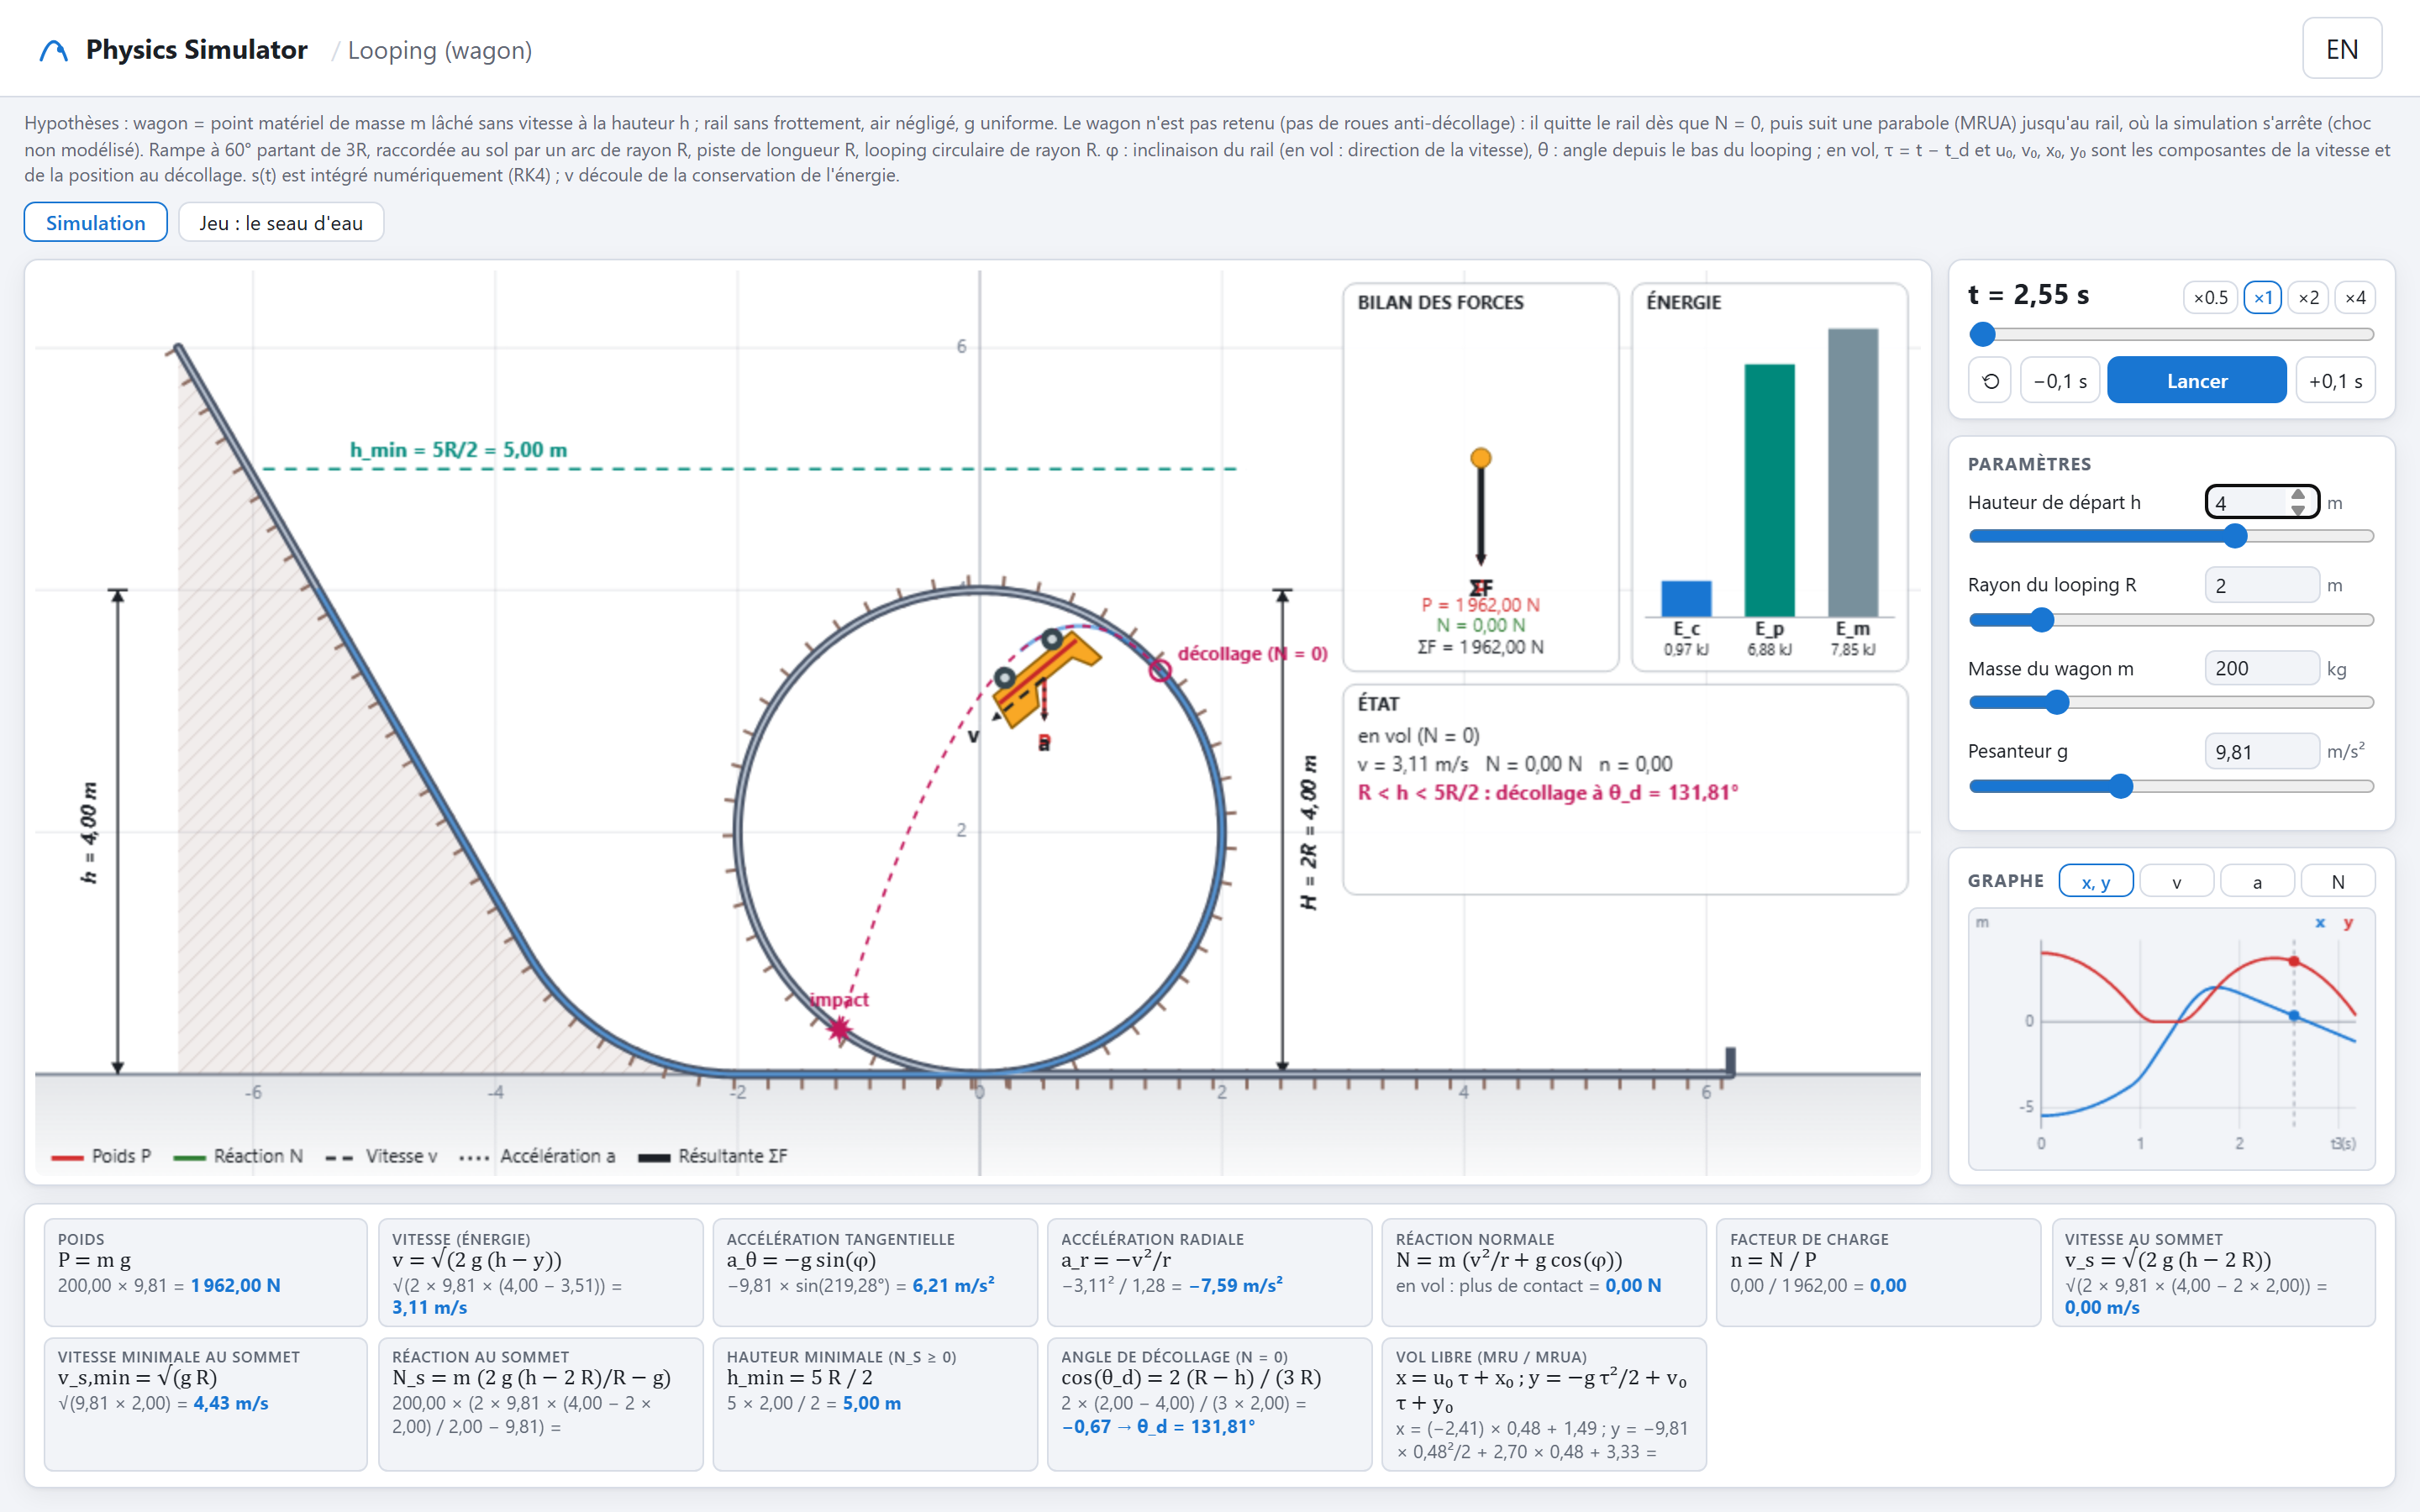
\includegraphics[width=\linewidth]{figures/captures/looping-decollage.png}
    \caption{\(h = 4\) m pour \(R = 2\) m : décollage prévu à
      \(\theta_d = \ang{131,81}\), parabole en tirets jusqu'à l'impact.}
  \end{subfigure}\hfill
  \begin{subfigure}[b]{0.27\linewidth}
    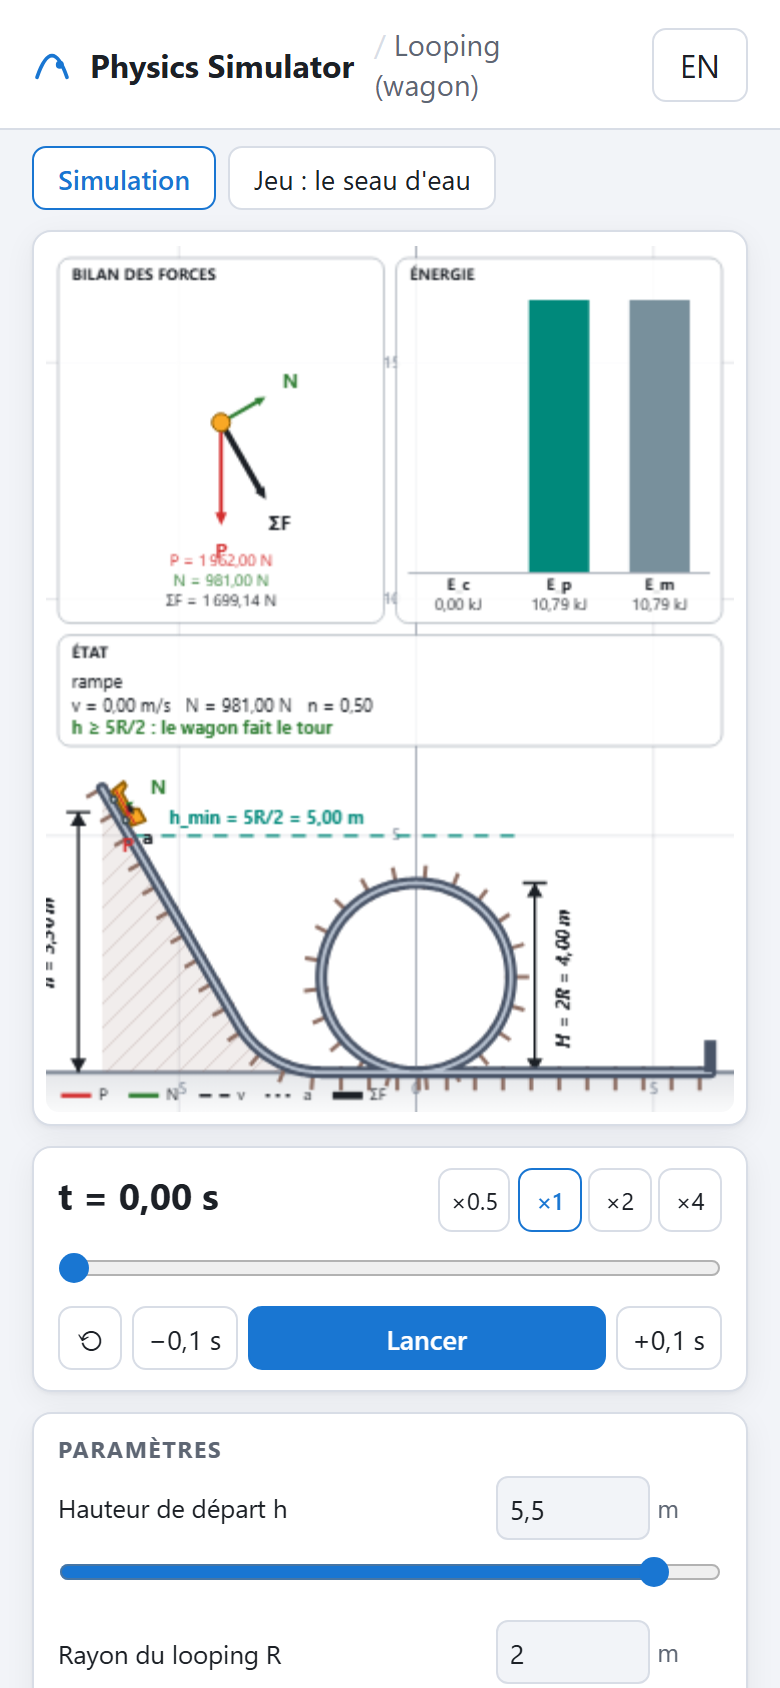
\includegraphics[width=\linewidth]{figures/captures/looping-telephone.png}
    \caption{Même page sur téléphone : bandeau d'informations au-dessus du rail.}
  \end{subfigure}
  \caption{Cas du décollage (\(R < h < 5R/2\)) et adaptation à un écran étroit.}
  \label{fig:wagon-decollage}
\end{figure}

\section{Le mode jeu : principe commun}

\begin{arediger}{1 page}
Règles communes à tous les jeux : une seule grandeur libre, situation tirée au
hasard mais \emph{prouvablement soluble} (génération constructive autour d'une
solution de référence, vérificateur pur, tirage par rejet, cas de repli),
paliers 1, 5, 10, 20, 40, 70, 100, formules et graphes cachés, mise en page
identique au mode normal. Le jeu du looping est détaillé au chapitre suivant.
\end{arediger}
